\section{Beyond the Standard Model}
Over the years, many theories have been developed to solve one or more of the SM shortcomings, but so far none of these theories have found experimental support yet. In the following sections, some of these scenarios for physics beyond the SM are reviewed, with a focus on those predicting new phenomena of interest for this dissertation.

\subsection{Supersymmetry} 
Supersymmetric models introduce a new symmetry, referred to as ``supersymmetry'' (SUSY), which transforms a bosonic state into a fermionic state and viceversa, being the last possible extension of the Lorentz group \cite{Haag:1974qh,Drees:1996ca}. This symmetry introduces a superpartner for each SM particle. The existence of those partners can stabilise the Higgs-boson mass, solving the hierarchy problem. In fact, if a new boson $S$, which couples to the Higgs boson, is introduced for each fermion $f$ the correction to the Higgs-boson mass due to this boson will be:

\be
\delta m_{H}^{2}=\frac{y^{2}_{S}}{16\pi^{2}}\left[2\Lambda^{2}+\mathcal{O}\left( m_{S}^{2}\ln\left( \frac{\Lambda}{m_{S}}\right) \right) \right].
\ee  

\noindent Bose-Einstein statistics implies an opposite sign with respect to the fermion mass correction shown in equation \ref{sec:theo:eq:higgcorr}. Therefore, if $y_{S} = |y_{f}|$, each of the fermion terms have a counter term that naturally cancels the quadratic divergence introduced. The residual correction left, ignoring the logarithmic contribution, is proportional to the quadratic mass difference between the fermion and the boson:

\be
\delta m_{H}^{2}=\frac{y^{2}_{f}}{16\pi^{2}}|m_{S}^{2}-m_{f}^{2}|.
\ee

\noindent According to the the ``naturalness'' argument, these corrections must not be much greater than $m_{H}$ in order to avoid too much fine tuning. This argument, not strict but quite desirable, sets the scale of the SM validity around the $\tev$, where the supersymmetric theory would replace the SM up to the Plank scale. Supersymmetry naturally predicts superpartners with the  same mass as the SM particles but, since no supersymmetric particles have been observed yet, supersymmetry must be a broken symmetry at low energy \cite{Martin:1997ns,Witten:1981nf} and so the masses of the superpartners have to be beyond the reach of current experiments.\par
Supersymmetry is not a fixed model but rather a framework that allows many SM extensions depending on the number of generators in the symmetry group, as well as the composition and arrangement of the SM particles into supermultiplets. The Minimal Supersymmetric SM (MSSM) is a model that introduces the minimal number of new particles. It obeys to the same gauge symmetry of the SM, but it doubles the spectrum of particles, since for every partner of the SM, a superpartner is postulated, differing by half a unit of spin. Spin-0 superpartners of the fermions are denoted starting with an extra ``s'' (e.g. the selectron is the superpartner of the electron) while the spin-1/2 superpartners of the bosons are added the suffix ``ino'' (e.g. the gluino is the superpartner of the gluon). Table \ref{sec:theo:tab:MSSM_content} summarises the MSSM particle content. 

\begin{table}[!ht]
  \begin{center}
    \begin{small}
      %\setlength{\tabcolsep}{0.0pc}
      %\begin{tabular*}{\textwidth}{@{\extracolsep{\fill}}ccccc}
      \begin{tabular}{ccccc}
        \toprule
        \toprule
        \textbf{Names} & \textbf{Spin} & \textbf{\boldmath{$P_R$}} & \textbf{Gauge eigenstates}      & \textbf{Mass Eigenstates} \\
        \midrule
        Higgs bosons   & $0$           & $+1$                 & $H_u^0$ $H_d^0$ $H_u^+$ $H_d^-$ & $h^0$ $H^0$ $A^0$ $H^\pm$ \\
        \midrule
        \multirow{3}{*}{Squarks} & \multirow{3}{*}{$0$} & \multirow{3}{*}{$-1$} & $\tilde{u}_L$ $\tilde{u}_R$ $\tilde{d}_L$ $\tilde{d}_R$ & same \\
        &                      &                       & $\tilde{s}_L$ $\tilde{s}_R$ $\tilde{c}_L$ $\tilde{c}_R$ & same \\
        &                      &                       & $\tilde{t}_L$ $\tilde{t}_R$ $\tilde{b}_L$ $\tilde{b}_R$ & $\tilde{t}_1$ $\tilde{t}_2$ $\tilde{b}_1$ $\tilde{b}_2$ \\
        \midrule
        \multirow{3}{*}{Sleptons}& \multirow{3}{*}{$0$} & \multirow{3}{*}{$-1$} & $\tilde{e}_L$ $\tilde{e}_R$ $\tilde{\nu}_e$ & same \\
        &                      &                       & $\tilde{\mu}_L$ $\tilde{\mu}_R$ $\tilde{\nu}_\mu$ & same \\
        &                      &                       & $\tilde{\tau}_L$ $\tilde{\tau}_R$ $\tilde{\nu}_\tau$& $\tilde{\tau}_1$ $\tilde{\tau}_2$ $\tilde{\nu}_\tau$ \\
        \midrule
        Neutralinos    & $1/2$           & $-1$                 & $\tilde{B}^0$ $\tilde{W}^0$ $\tilde{H}_u^0$ $\tilde{H}_d^0$ & $\tilde{\chi}^{0}_{1}$ $\tilde{\chi}^{0}_{2}$ $\tilde{\chi}^{0}_{3}$ $\tilde{\chi}^{0}_{4}$ \\
        \midrule
        Charginos      & $1/2$           & $-1$                 & $\tilde{W}^\pm$ $\tilde{H}_u^+$ $\tilde{H}_d^-$ & $\tilde{\chi}^{\pm}_{1}$ $\tilde{\chi}^{\pm}_{2}$ \\
        \midrule
        Gluino         & $1/2$           & $-1$                 & $\tilde{g}$ & same \\
        \bottomrule
        \bottomrule
      \end{tabular}
    \end{small}
  \end{center}
  \caption[Predicted MSSM spectra.]{The predicted particle spectra in the MSSM (sfermion mixing for the first two families is assumed to be negligible).}
  \label{sec:theo:tab:MSSM_content}
\end{table}

The Higgs sector is enlarged in the MSSM with the introduction of an additional complex doublet, leading to five physical Higgs bosons after the SSB mechanism. Baryonic and leptonic number violating terms are included in the most general MSSM, but strong constraints on those terms come from the fact that no such violations have been observed. A new discrete symmetry, $R$-parity, is added to avoid such terms and the conserved quantum number is defined as:

\be
P_{R}=(-1)^{3(B-L)+2s},
\ee 

\noindent where $B$ and $L$ refer to the baryon and lepton quantum numbers respectively, and $s$ is the spin of the particle. This definition sets all the SM particles and the Higgs bosons to have $P_{R} = +1$, while their SUSY partners have $P_{R} =-1$. $R$-parity is not necessarily conserved but, when is imposed as a discrete symmetry, it has the consequence that SUSY particles are always produced in pairs. Furthermore, the lightest supersymmetric particle must be stable since, due to the conservation of $R-$parity, it cannot decay into ordinary particles, thus providing a good candidate for dark matter. The MSSM solves in an elegant way the hierarchy problem, provides a candidate for dark matter, can predict enough CP violation to explain baryon asymmetry and, finally, predicts the unification of the three SM gauge couplings. On the other hand, it introduces 105 new parameters, to be added to the 19 parameters of the SM. In order to reduce the number of parameters to be considered, several simplifications and assumptions are introduced in collider searches. Usually, only the sparticles that contribute to a particular final state are considered. The rest of the superpartners are considered heavy enough so that they can be completely decoupled. 

\subsubsection{The Two-Higgs-doublet model} 
\label{sec:theo:hdm}

In supersymmetric theories the scalars belong to chiral multiplets and their complex conjugates belong to multiplets of the opposite chirality; a single Higgs doublet is unable to give mass simultaneously to the charge $+2/3$ and charge $-1/3$ quarks  since multiplets of different chiralities cannot couple together in the Lagrangian. Thus, the MSSM contains two Higgs doublets.\par
A simple possible extension of the SM, without invoking the presence of supersymmetry, is the introduction of two complex Higgs doublets instead of one:

\be
\Phi_{1}=\begin{pmatrix} \phi^{+}_{1}\\ \phi^{0}_{1}\\ \end{pmatrix}, \,\,\,\,\,\,\,\,\, \Phi_{2}=\begin{pmatrix} \phi^{-}_{2}\\ \phi^{0}_{2}\\ \end{pmatrix},
\ee

\noindent where $\Phi_{1}$ and $\Phi_{2}$ have positive hypercharge like the SM doublet, and the superscripts $\pm$ and $0$ denote the electric charge of the scalar fields $\phi$. The class of models that include two Higgs doublets is referred to as Two-Higgs-Doublet Model (2HDM) \cite{Branco:2011iw}. These models can explain the baryon asymmetry in the universe due to the flexibility of their scalar mass spectrum \cite{Trodden:1998qg} and the existence of additional sources of CP violation \cite{Eriksson:2009ws}. Those models can as well rotate away the CP-violating term in the QCD Lagrangian. Assuming that CP is conserved in the Higgs sector and that discrete symmetries eliminate from the potential all quartic terms odd in either of the doublets, the most general scalar potential is:

\begin{equation}
\begin{split}
&V= m_{11}^{2}\Phi_{1}^{\dagger}\Phi_{1}+m_{22}^{2}\Phi_{2}^{\dagger}\Phi_{2}-m_{12}^{2}(\Phi_{1}^{\dagger}\Phi_{2}+\Phi_{2}^{\dagger}\Phi_{1})+\frac{\lambda_{1}}{2}(\Phi_{1}^{\dagger}\Phi_{1})^{2}+\\
&+\frac{\lambda_{2}}{2}(\Phi_{2}^{\dagger}\Phi_{2})^{2}+\lambda_{3}\Phi_{1}^{\dagger}\Phi_{1}\Phi_{2}^{\dagger}\Phi_{2}+\lambda_{4}\Phi_{1}^{\dagger}\Phi_{2}\Phi_{2}^{\dagger}\Phi_{1}+\frac{\lambda_{5}}{2}\left[(\Phi_{1}^{\dagger}\Phi_{2})^{2}+(\Phi_{2}^{\dagger}\Phi_{1})^{2} \right],
\end{split}
\end{equation}

\noindent where all parameters are real. The minimisation of the potential gives:
\be
\langle \Phi_{1} \rangle = \begin{pmatrix} 0\\ \frac{v_{1}}{\sqrt{2}}\\ \end{pmatrix}, \,\,\,\,\,\,\,\, \langle \Phi_{2} \rangle = \begin{pmatrix} 0\\ \frac{v_{2}}{\sqrt{2}}\\ \end{pmatrix},
\ee

\noindent and excitations of the different Higgs fields around their VEVs can be expressed as:
\be
\Phi_{1}=\begin{pmatrix} \phi^{+}_{1}\\ (v_1+\rho_1+i\eta_1)/\sqrt{2}\\ \end{pmatrix}, \,\,\,\,\,\,\,\,\, \Phi_{2}=\begin{pmatrix} \phi^{-}_{2}\\ (v_2+\rho_2+i\eta_2)/\sqrt{2} \\ \end{pmatrix},
\ee
\noindent with $\rho_{i}={\rm Re}(\phi_{i}^{0})-v_{i}$ and $\eta_i={\rm Im}(\phi_{i}^{0})$, $i=1,2$.
From these eight fields three of them are absorbed to generate the mass of the $W$ and $Z$ bosons and the remaining five correspond to physical Higgs fields: two CP-even scalars $h$ and $H$ with $m_h<m_H$, a pseudoscalar (CP-odd) $A$, and two charged scalars $H^{\pm}$.
The angles $\alpha$ and $\beta$ are the rotation angles that diagonalise the mass-squared matrix of the scalars, and the one of the charged scalars and of the pseudoscalars respectively. The single most important parameter of the 2HDM is:
\be
\tan\beta\equiv\frac{v_2}{v_1},
\ee 
\noindent the ratio of the VEVs of both Higgs doublets. The two parameters $\alpha$ and $\beta$ determine the interactions of the various Higgs fields with the vector bosons and with the fermions; they are thus crucial in discussing the phenomenology of a 2HDM. A feature of 2HDMs is the possibility of tree-level flavour-changing neutral currents (FCNC) \cite{Branco:2011iw}. It is possible to remove FCNCs from the theory by forcing (with the introduction of discrete symmetries) any given type of fermions to couple to not more than one doublet \cite{Glashow:1976nt}. Table \ref{chp:the:tab:2hdm} shows the possible combinations usually denoted as Type I to Type IV. 


\begin{table}[htb!]
\begin{center}
  \begin{tabular}{c c c c c}
  \hline  
  &Type I& Type II&Type III&Type IV\\
   \hline
   $q^{i}_{R_{u}}$ & $\phi_2$ & $\phi_2$ & $\phi_2$ & $\phi_2$\\
   $q^{i}_{R_{d}}$ & $\phi_2$ & $\phi_1$ & $\phi_2$ & $\phi_1$\\
   $\ell^{i}_{R}$ & $\phi_2$ & $\phi_1$ & $\phi_1$ & $\phi_2$\\
\hline
\end{tabular}

\captionsetup{width=0.85\textwidth} \caption{\small 2HDM Types defined using the fermions fields $q^{i}_{R_{u}}$, $q^{i}_{R_{d}}$ and $\ell^{i}_{R}$ and their coupling to the Higgs doublets $\Phi_1$ and $\Phi_2$.}
\label{chp:the:tab:2hdm}
\end{center}
\end{table}


\subsection{Extra dimensions} 

Several theories propose a spacetime with more than 3+1 dimensions to address some of the shortcomings of the SM. The idea is sketched in figure \ref{sec:theo:fig:extradim}: the vertical dimension stands for the 3+1 (infinitely large) dimensions and the fifth dimension is finite, being compactified on a circle of radius $R$. Our world would correspond to the surface of the cylinder, usually referred to as the ``brane''. These extra-dimensional models are built to be consistent with all aspects of the SM and the presence of the extra dimension can explain, for example, the apparent weakness of the gravitational force, making gravity diluted in the extra dimensions. The higher-dimensional space is usually referred to as the ``bulk'' and particles propagating in the compactified extra dimension manifest in a four-dimensional brane as an infinite number of Kaluza-Klein (KK) modes. Extra-dimensional models are classified according to the geometry of the extra dimension: flat or warped.


\bfig[h!]
\centering
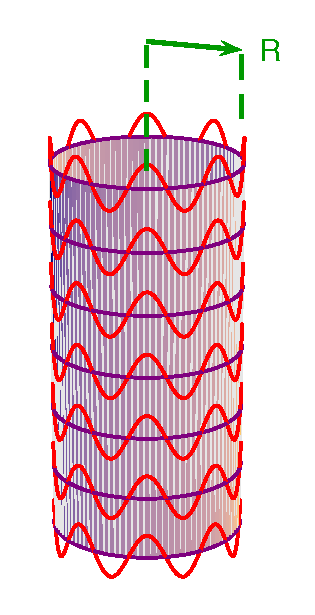
\includegraphics[width=0.2\textwidth]{figures/Theory/extradim.eps}
\captionsetup{width=0.85\textwidth} \caption{\small Representation of an extra spatial dimension with radius $R$. From reference \cite{Ponton:2012bi}.}
\label{sec:theo:fig:extradim}
\efig


\subsubsection{Flat-extra-dimensions models} 

In this category of models there are Arkani-Hamed-Dimopoulos-Dvali (ADD) models \cite{ArkaniHamed:1998rs} in which the extra dimension is accessible only to gravity; therefore, the only particle propagating in the bulk is the graviton. It requires two or more extra dimensions with a size $R$ that can range between $\sim1$ mm and $\sim1$ \tev$^{-1}$. The ``effective'' $4D$ Planck mass as a function of the $D$-dimensional parameters can be expressed as:
\be
M_{P}^{2}= M_{D}^{2+n}R^{n},
\ee
\noindent where $M_{D}$ is Planck scale in $D=4+n$ dimensions.  Fixing $M_{D}$ at around the electroweak scale to avoid introducing a new scale in the model, many options for the number and the size of the extra dimensions are possible. However, experimental lower bounds on the $M_{D}$ scale for ADD models are in the range of $4-6$ $\tev$ for $2-6$ extra dimensions \cite{Aaboud:2016tnv}, pushing $M_{D}$ away from the electroweak scale. \par
Allowing SM particles to propagate in the bulk is a feature of Universal Extra-Dimensional (UED) models \cite{Appelquist:2000nn}. The main challenge for these theories is recovering the SM behavior after compactification of the extra dimensions. One possibility is the existence of two extra dimensions, which are compactified under the real projective plane geometry (RPP) \cite{Burdman:2006gy,Cacciapaglia:2009pa}, referred to as 2UED/RPP model. In this case, new states can be produced only in pairs and the lightest KK state is stable, leading to a candidate for dark matter.

\subsubsection{Warped-extra-dimension models} 
\label{sec:theo:warped}

Randall and Sundrum (RS) \cite{Randall:1999vf,Contino:2006nn} models use a warped geometry in a five-dimensional Anti-de Sitter (AdS) spacetime with a compactification scale $\sim$\tev. The origin of the huge difference between the electroweak scale and the Planck scale is explained by the gravitational redshift factor present in the warped AdS metric. The ``warp'' factor determines how $4D$ scales change as a function of the position in the extra dimension:  energy scales for $4D$ fields localised on the infrared (IR) brane are red-shifted compared to the ones on the ultraviolet (UV) brane. Therefore, a natural solution to the hierarchy problem \cite{Randall:1999ee} can be achieved in this framework if the Higgs field is localised on the IR brane where the effective mass scales are of order \tev, while SM gauge bosons and fermions can propagate in the $5D$ bulk. In warped-extra-dimension models the Higgs boson appears as the fifth component of a $5D$ gauge boson and its mass is protected by the $5D$ gauge invariance.  In these models there is a light Higgs boson whose mass can be around 125 \gev, but it behaves as a composite pseudo-Nambu-Goldstone boson (see section \ref{sec:theo:compositeness}) with couplings that deviate from those of the SM Higgs boson.


\subsection{Compositeness}
\label{sec:theo:compositeness}

Several times a particle that was believed elementary revealed its composite nature when studied at higher energy scales, e.g. pions, protons and
even atoms were considered elementary at some point. Nowadays the idea that some of the SM particles may be composite is a fascinating  one, as the discovery of compositeness would radically redefine most of the fundamental questions in particle physics.\par
This idea developed starting from the not exact (i.e.~broken) chiral symmetry in QCD, which produces three Goldstone bosons with a mass, usually referred to as pseudo-Nambu-Goldstone Bosons (PNGB). The three PNGBs are the pions, which are not elementary particles and have a naturally low mass compared to other mesons. Before it was established as a meson, i.e. a quark-antiquark bound state of the strong interaction, the neutral pion was considered an elementary
particle, responsible for mediating the strong interaction. The low mass ($\sim$100 \mev) of the neutral pion could, however, not be explained without interpreting it as a meson. This in turn required new particles at the $\gev$ scale, which were indeed found thereafter. This is the result of strong dynamics that can be reinterpreted in terms of more fundamental degrees of freedom, the quarks.\par
Some new theories propose that the Higgs boson is a composite PNGB \cite{Agashe:2004rs,Kaplan1984187,Fukano:2013aea,Contino:2010rs}. In these theories, a new strongly-interacting sector with a new global symmetry is present at the compositeness scale, usually $\sim\tev$. A composite light Higgs boson emerges, much like the pion of QCD, as the PNGB of a global symmetry breaking of that sector. The explicit symmetry breaking is induced by interactions of the SM gauge bosons and fermions with the strong sector. Loops of SM fermions and gauge bosons generate a Higgs potential that eventually breaks the electroweak symmetry at scale $v$, generated dynamically and lower than the strong sector (compositeness) breaking scale. In this scenario the radiative corrections to the Higgs boson mass do not reach the Planck scale since the Higgs boson will reveal its composite nature at the energy scale of the new strong sector. Strongly-interacting theories usually are subject to stringent constraints from precision electroweak data, but weakly-coupled models such as the one in section \ref{sec:theo:warped} can satisfy such bounds. \par
Some other theories propose instead that the top quark is composite \cite{Pomarol:2008bh}, made of some new constituent particles (``preons'') bound together by a new confining force, or a condensed state. Most of those models \cite{Lillie:2007hd,Kumar:2009vs} focus on right-handed top quarks to avoid strong constraints from precision electroweak data.\\


\subsection{Vector-like quarks}
\label{sec:theo:vlq}

A fermion is vector-like if  left- and right-handed chiralities belong to the same representation of the symmetry group of the underlying theory.
Vector-like quarks (VLQs) are triplets under the $SU(3)_{C}$ gauge group, and so their left- and right-handed components carry the same colour and electroweak quantum numbers \cite{Aguilar-Saavedra:2013qpa,Okada:2012gy,Aguilar-Saavedra:2013wba,jaas}. VLQs have been introduced in many different BSM scenarios; in composite Higgs models VLQs are part of the condensate that drives the EW symmetry breaking, the excited partners of SM quarks in extra-dimensional models are also vector-like. The presence of VLQs can introduce new sources of CP violation to solve the baryon asymmetry \cite{delAguila:1997vn} and can also explain the observed $A^{b}_{FB}$ asymmetry through mixing with the bottom quark \cite{Choudhury:2001hs,Kumar:2010vx}. The introduction of VLQs also stabilises the Higgs boson mass since the quadratic divergences cancel and only a logarithmic divergence remains. The one-loop contributions to the Higgs boson mass are shown in figure \ref{fig:theo:VLQHiggsmass}. 

\begin{figure}[h!]
\begin{subfigure}{0.33\textwidth}
  \centering
  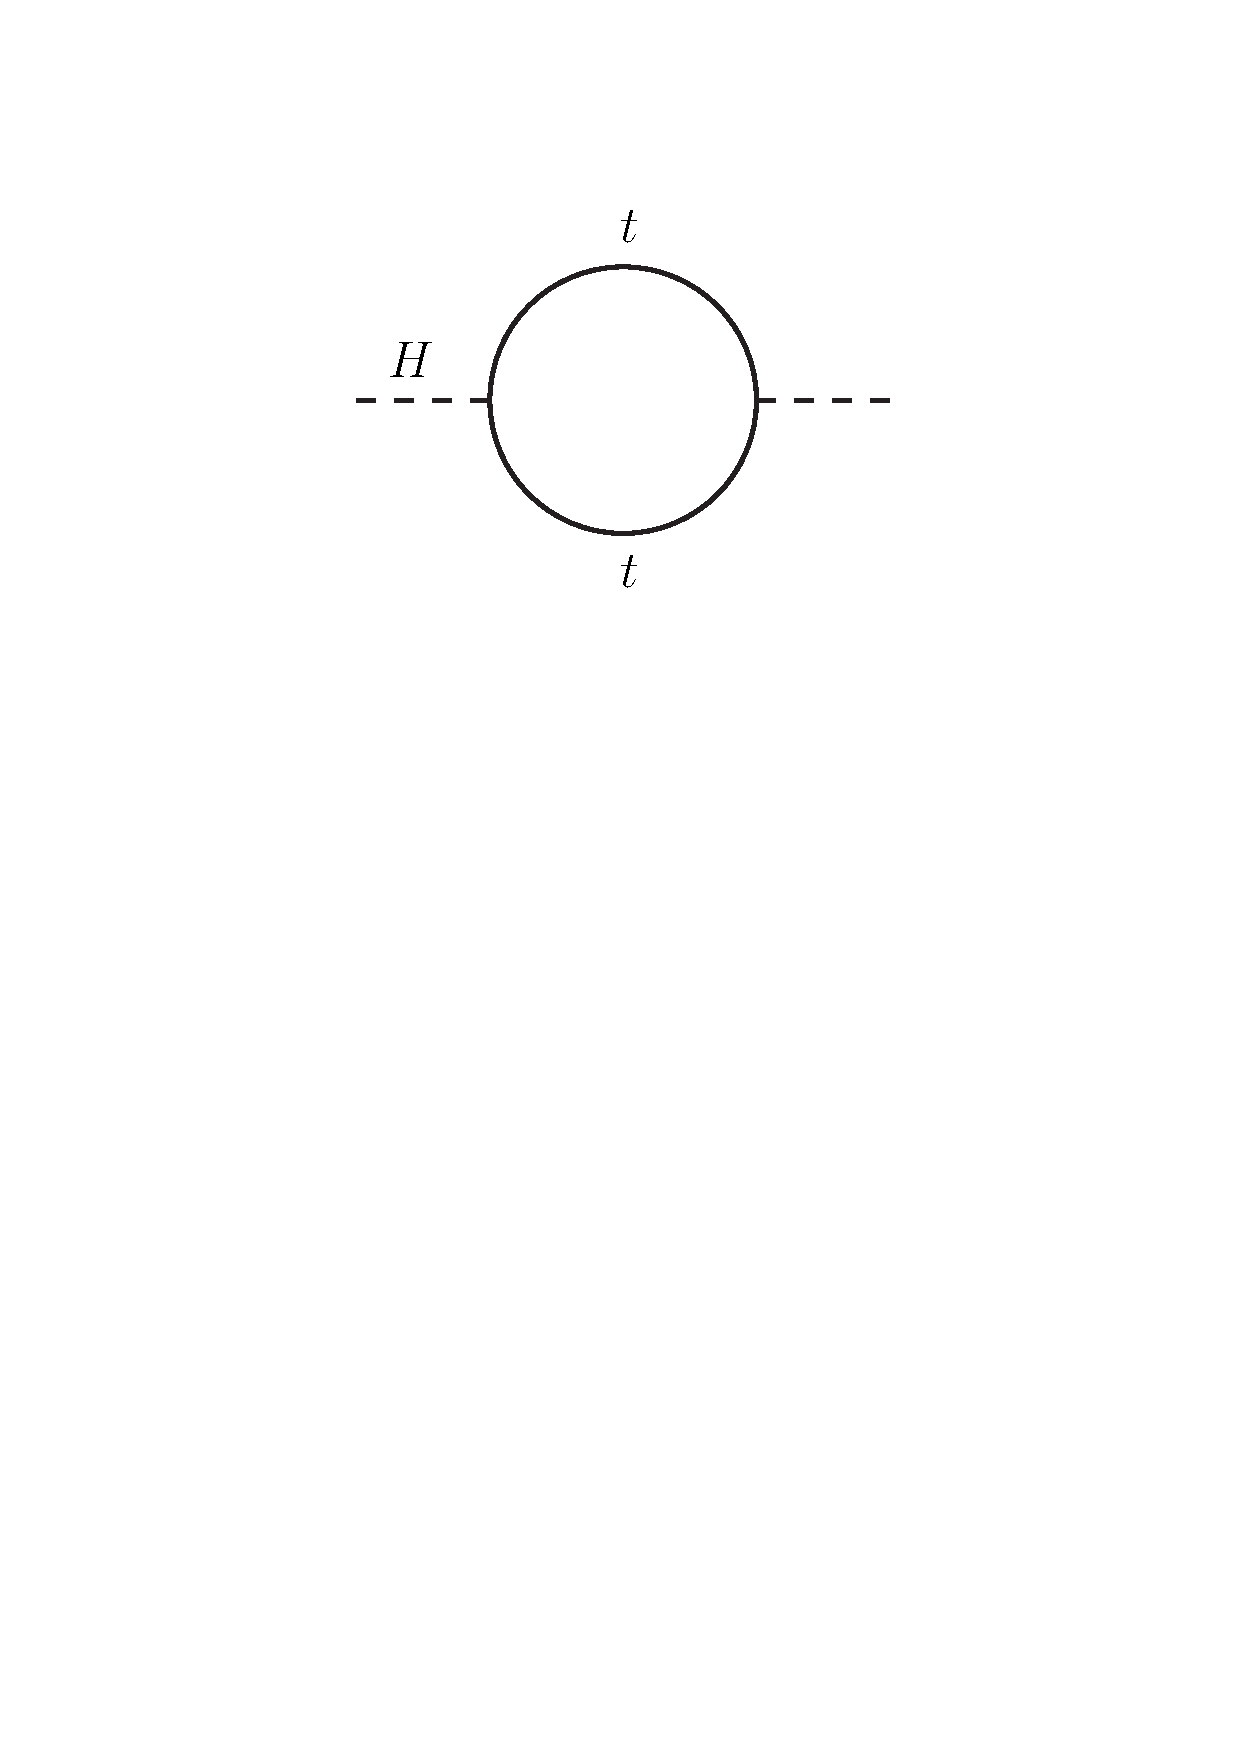
\includegraphics[width=0.9\textwidth]{figures/Theory/loop_toptop_good.pdf}
  \caption{}
  \label{}
\end{subfigure}
\begin{subfigure}{0.33\textwidth}
  \centering
  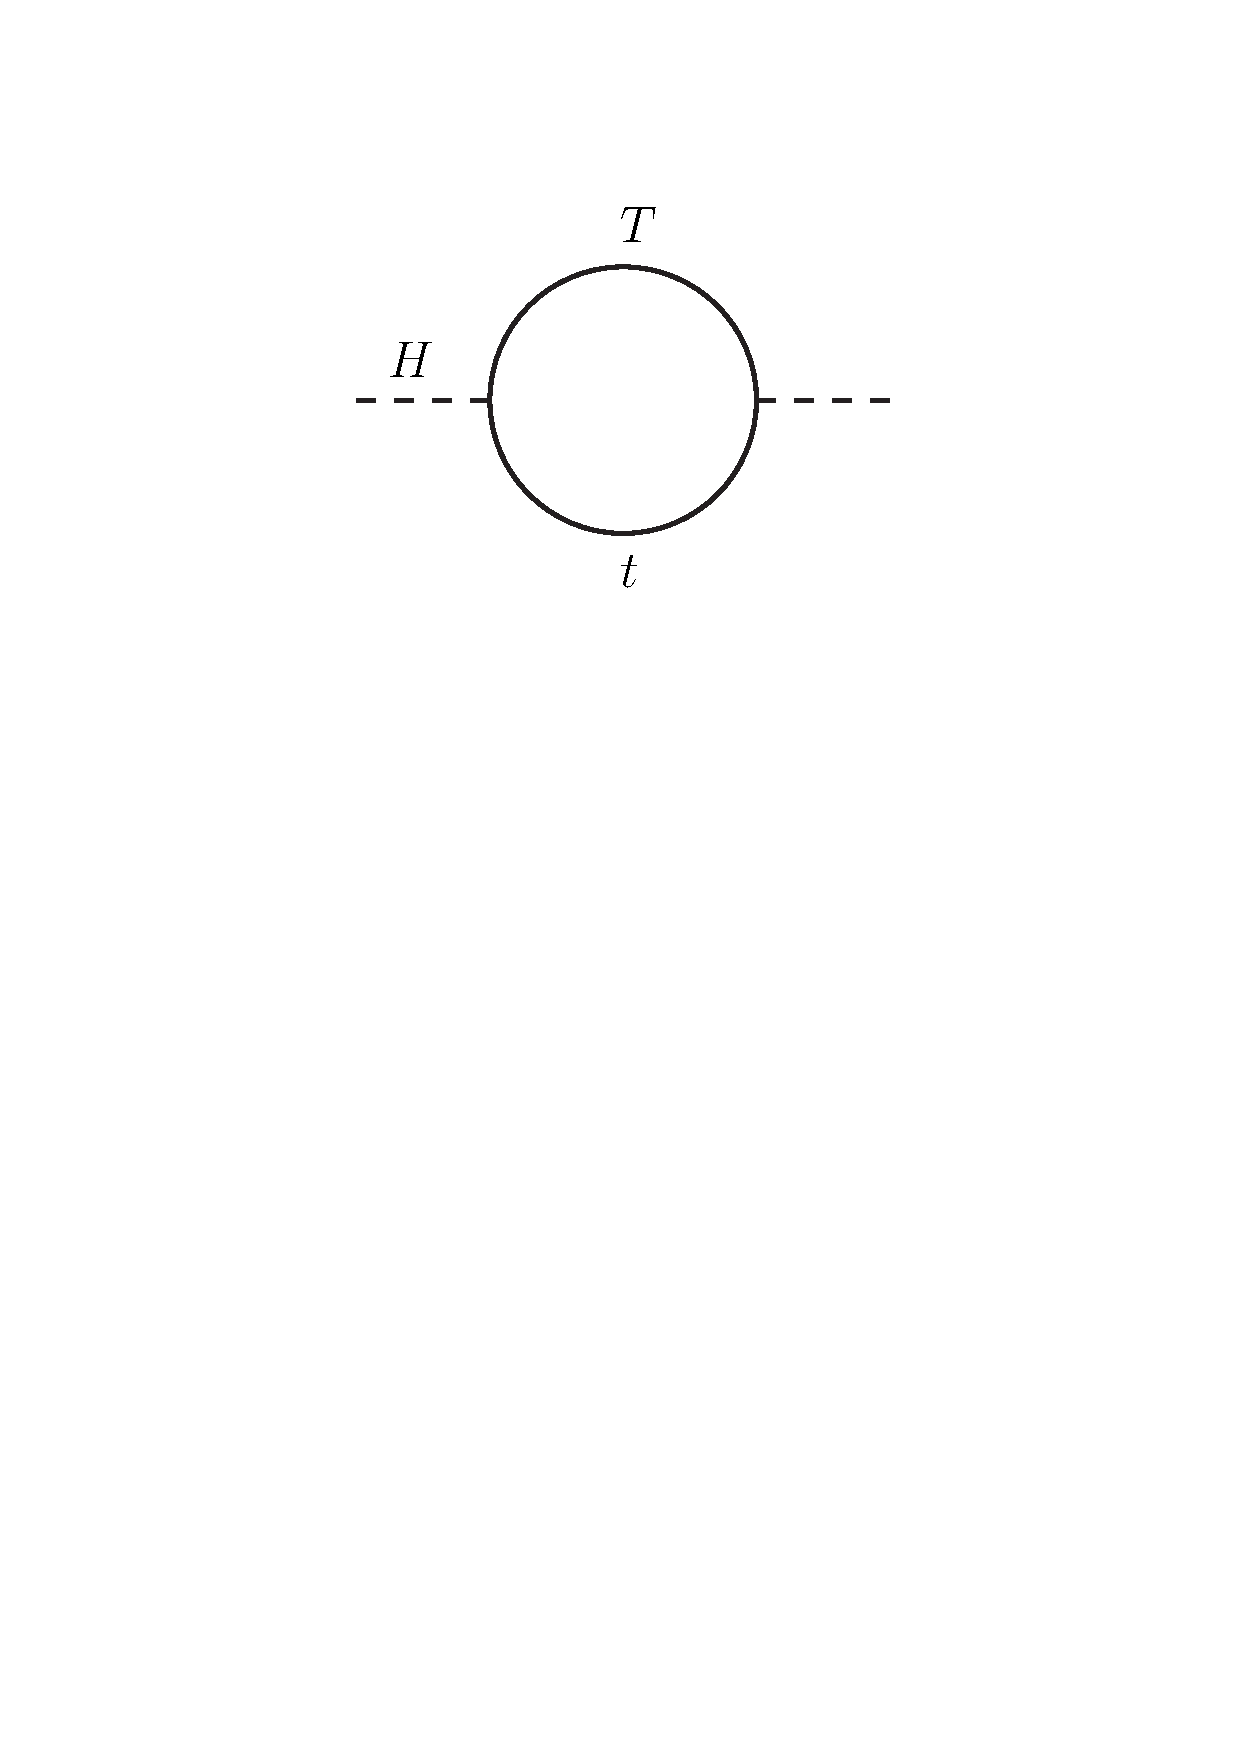
\includegraphics[width=0.9\textwidth]{figures/Theory/loop_topT_good.pdf}
  \caption{}
  \label{}
\end{subfigure}
\begin{subfigure}{0.33\textwidth}
  \centering
  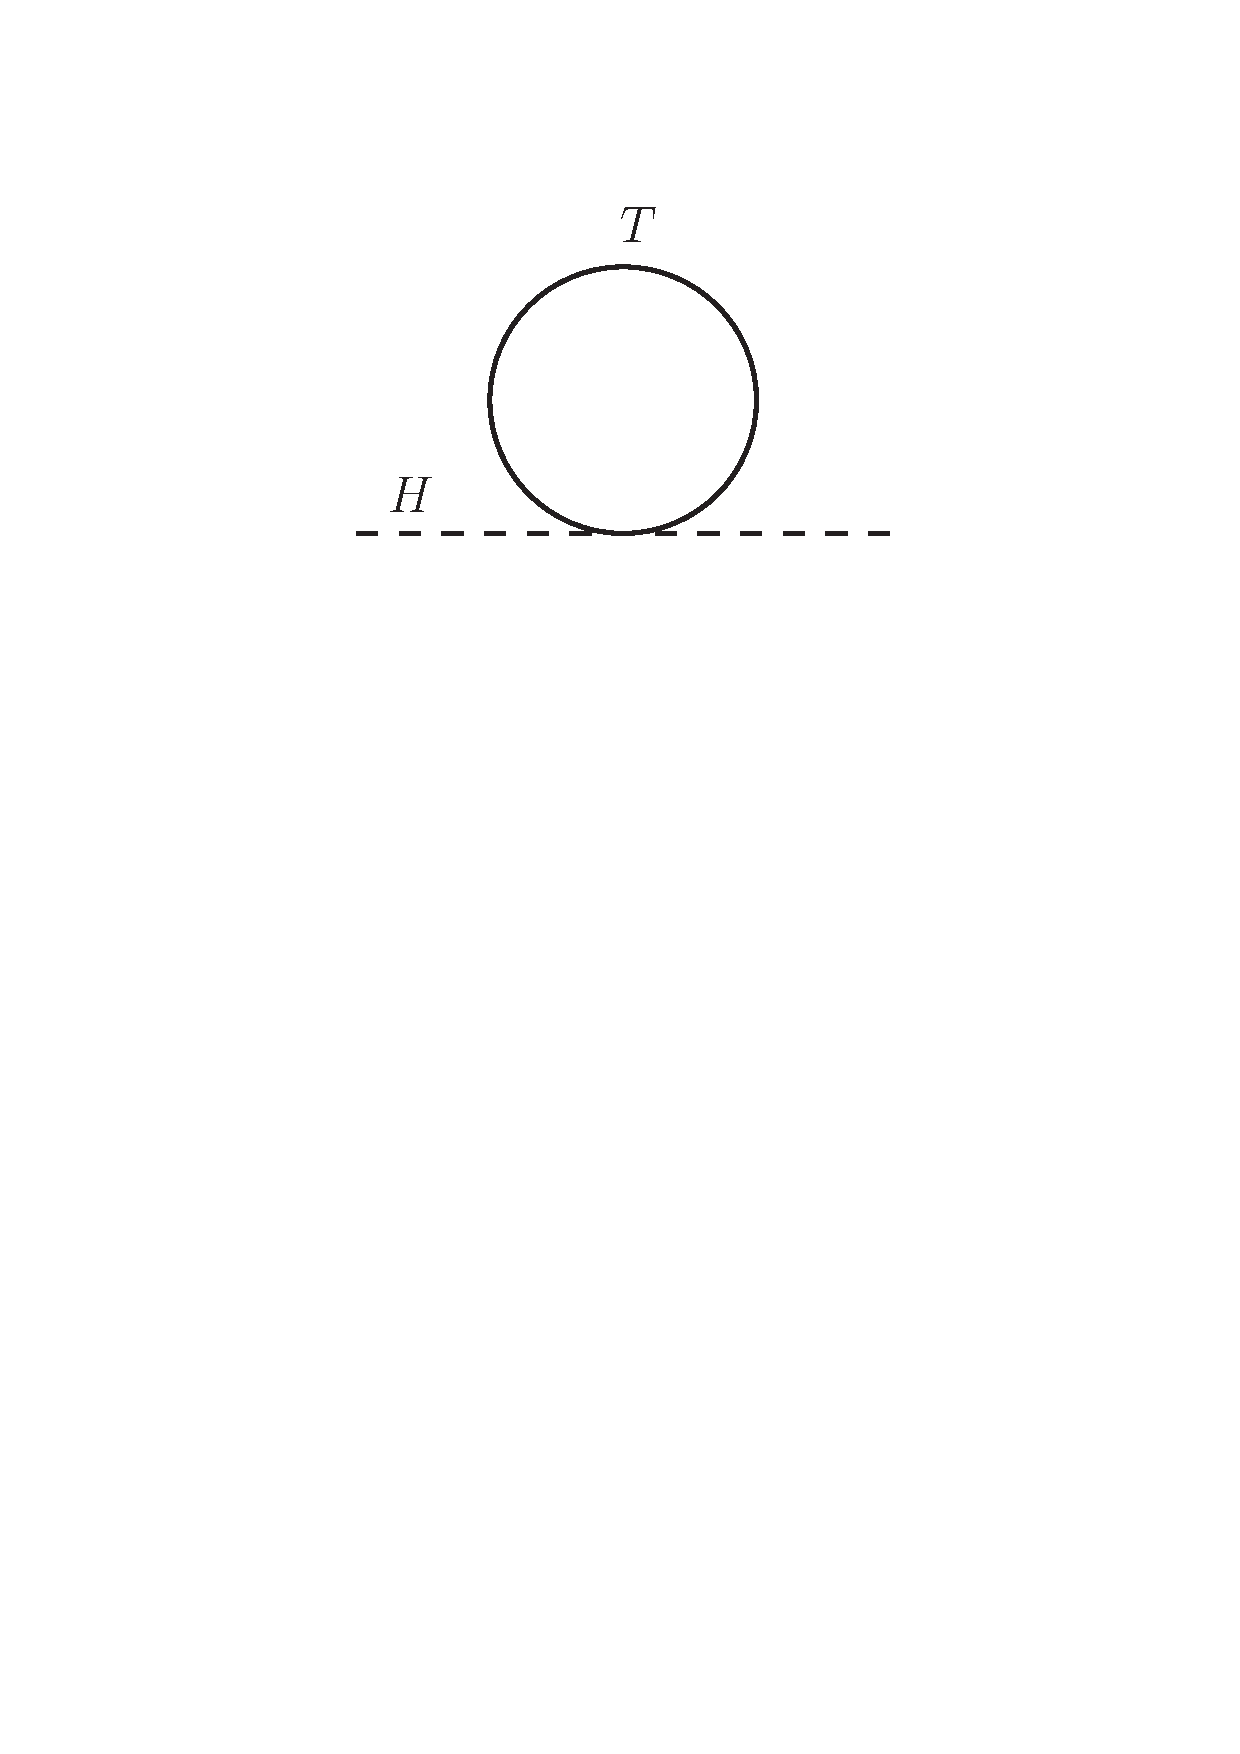
\includegraphics[width=0.9\textwidth]{figures/Theory/loop_T_good.pdf}
  \caption{}
  \label{}
\end{subfigure}

\captionsetup{width=0.85\textwidth} \caption{\small One-loop contributions to the Higgs boson mass term from (a) the top quark and (b, c) a vector-like top-quark partner $T$.}
\label{fig:theo:VLQHiggsmass}
\end{figure}

The mass term $m_{f}\bar{\Psi}_{f}\Psi_{f}$ of a VLQ $f$ is gauge invariant under $SU(2)_{L} \otimes U(1)_{Y}$, i.e. its mass is generated without the need for a Yukawa interaction with the Higgs boson. Therefore, there are no constraints on the existence of VLQs arising from the measured Higgs-boson production cross section, since the contribution to loop-induced Higgs-boson couplings, $ggH$ and $\gamma\gamma H$, is suppressed by the heavy quark mass.
Classifying VLQs in multiplets of $SU(2)_{L}$, it is possible to write gauge-invariant interaction terms only for singlets, doublets and triplet representations, shown in table \ref{sec:theo:vlqs}. 

\begin{table}[htb]
\begin{eqnarray*}
\setlength{\arraycolsep}{2pt}
\begin{array}{cccccccc}
&\multicolumn{2}{c}{\mbox{Singlets}}&\multicolumn{3}{c}{\mbox{Doublets}}&\multicolumn{2}{c}{\mbox{Triplets}}\\
& 
\begin{array}{c} ~ \\ (U) \\ ~ \\ ~ \end{array} &
\begin{array}{c} ~ \\ ~ \\ (D) \\ ~ \end{array} & 
\begin{array}{c} \left(\begin{array}{c} X \\ U \end{array}\right) \\ ~ \\ ~ \end{array} &
\begin{array}{c} ~ \\ \left(\begin{array}{c} U \\ D \end{array}\right) \\ ~ \end{array} &
\begin{array}{c} ~ \\ ~ \\ \left(\begin{array}{c} D \\ Y \end{array}\right) \end{array} & 
\begin{array}{c} \left(\begin{array}{c} X \\ U \\ D \end{array}\right) \\ ~ \end{array} &
\begin{array}{c} ~ \\ \left(\begin{array}{c} U \\ D \\ Y \end{array}\right) \end{array} \\
\midrule
Y/2  & 2/3 & -1/3 & 7/6 & 1/6 & -5/6 & 2/3 & -1/3 \\
\midrule
\mathcal{L}_{\rm Yukawa} &
\multicolumn{2}{c}{\begin{array}{c}-\lambda_u^i \bar q_L^i H^c U_R \\-\lambda_d^i \bar q_L^i H D_R \end{array}} &
\multicolumn{3}{c}{\begin{array}{c}-\lambda_u^i \psi_L H^{(c)} u_R^i \\-\lambda_d^i \psi_L H^{(c)} d_R^i \end{array}} &
\multicolumn{2}{c}{\begin{array}{c}-\lambda_i \bar q_L^i \tau^a H^{(c)} \psi_R^a \end{array}} \\
\midrule

\end{array} 
\end{eqnarray*}
\captionsetup{width=0.85\textwidth} \caption{\small VLQs in different $SU(2)_L$ representations with hypercharge quantum number and Yukawa mixing terms in the Lagrangian. Depending on the chosen representation, the Higgs boson may be $H$ or $H^c$; therefore, it has been noted as $H^{(c)}$ when necessary.}
\label{sec:theo:vlqs}
\end{table}


The mass eigenstates are labelled as $X$, $T$, $B$, and $Y$ with an electric charge of $+5/3$, $+2/3$, $-1/3$, $-4/3$ respectively.
The left-right symmetry of VLQs allows for tree-level flavour changing neutral currents, which are their distinctive feature.  In order to be consistent with precision electroweak data, a small mass splitting between VLQs belonging to the same $SU(2)_{L}$ multiplet is required \cite{Aguilar-Saavedra:2013qpa}, which forbids cascade decays such as $T \to WB$, and leaves direct decays into SM particles as the only possibility. VLQs interact with SM quarks and the Higgs boson through Yukawa couplings. VLQs can mix with the SM quarks; the mixing occurs in the left-handed sector for the singlet and triplet representations and in the right-handed sector for the doublet representation. The mixing of a VLQ and a SM quark is of the order $\sim m_{q}/M_{Q}$, where $M$ and $m$ are the masses of the VLQ and the SM quark respectively. Thus VLQs are expected to predominantly mix with the third SM generation, while mixing with lighter SM generations is mass suppressed. Under this assumption, the only possible decays for VLQs are into top / bottom quark plus a $W$, $Z$ or Higgs boson. For the quarks with exotic charges the only decay channels are $X \to W^{+}t$ and $Y\to W^{-}b$, while the heavy quarks  with charges $+2/3$ and $-1/3$ the possible channels are respectively:

\be
T\to W^{+}b,\, Zt,\, Ht \,\,\,\, \textrm{and} \,\,\,\, B\to W^{-}t,\, Zb,\, Hb.
\ee

\noindent The branching ratios for different channels have some dependence on the heavy quark masses and on the $SU(2)_{L}$ representation. For singlets all decay modes are possible, while for doublets the branching ratio depend on the relative size of the mixing factors $V_{Tb}$ and $V_{tB}$ of the extended CKM matrix. In this dissertation the scenario where $V_{Tb} \ll V_{tB}$ is assumed. Thus the mixing of the heavy quarks with the SM top quark is much stronger, and the $T\to Wb$ decay is suppressed, as well as $B\to Hb$ and $B\to Zb$. Table \ref{sec:theo:tab:VLQ_decay} summarises the possible decays modes for VLQs.
\begin{table}[htb!]
   \centering
   \begin{tabular}{ccc}
   \begin{tabular}{cc}
     \toprule
     \toprule
     Singlets & Decay modes \\
     \midrule
     & \\
     $X$ & $W^+t$ \\
     & \\
     $T$ & $W^+b,\, Ht,\, Zt$ \\
     & \\
     $B$ & $ W^-t,\, Hb,\, Zb$ \\
     & \\
     $Y$ & $W^-b$ \\
     & \\
     & \\%one empty line
     \bottomrule
     \bottomrule
   \end{tabular}

   & 

   \begin{tabular}{cc}
     \toprule
     \toprule
      Doublets & Decay modes\\
     \midrule
     &\\%one empty line
     \multirow{2}{*}{$\left(\begin{array}{c}X \\ T\end{array}\right)$} & $W^+t$\\
     & $Ht,\, Zt$\\
     &\\
     \multirow{2}{*}{$\left(\begin{array}{c}T \\ B\end{array}\right)$} & $ Ht,\, Zt$ \\%$W^+b,\, Ht,\, Zt$\\
     & $ W^-t$\\%$ W^-t,\, Hb,\, Zb$\\
     & \\
     \multirow{2}{*}{$\left(\begin{array}{c}B \\ Y\end{array}\right)$} & $Hb,\, Zb$\\
     & $W^-b$\\
     &\\%one empty line
     \bottomrule
     \bottomrule
   \end{tabular}
   & 

   \begin{tabular}{cc}
     \toprule
     \toprule
      Triplets & Decay modes\\
     \midrule
     &\\%one empty line
     \multirow{3}{*}{$\left(\begin{array}{c}X \\ T \\ B\end{array}\right)$} & $ W^+t$ \\
     & $W^+b,\, Ht,\ Zt$\\
     & $Hb,\, Zb$\\
     &\\%one empty line
     \multirow{3}{*}{$\left(\begin{array}{c}T \\ B \\ Y\end{array}\right)$} & $Ht,\, Zt$\\
     & $W^-t,\, Hb,\, Zb$\\
     & $W^-b$\\
     &\\%one empty line
     &\\%one empty line
     \bottomrule
     \bottomrule
   \end{tabular}
   \end{tabular}
   \captionsetup{width=0.85\textwidth} \caption{\small Allowed decay modes for vector-like singlets, doublets and triplets.}
     \label{sec:theo:tab:VLQ_decay}
   \end{table}
Figure \ref{fig:theo:VLQBRs} shows the decay branching ratios of the vector-like top and bottom partners for singlets and doublets as a function of the heavy-quark mass.
  
\begin{figure}[t!]
\begin{subfigure}{0.5\textwidth}
  \centering
  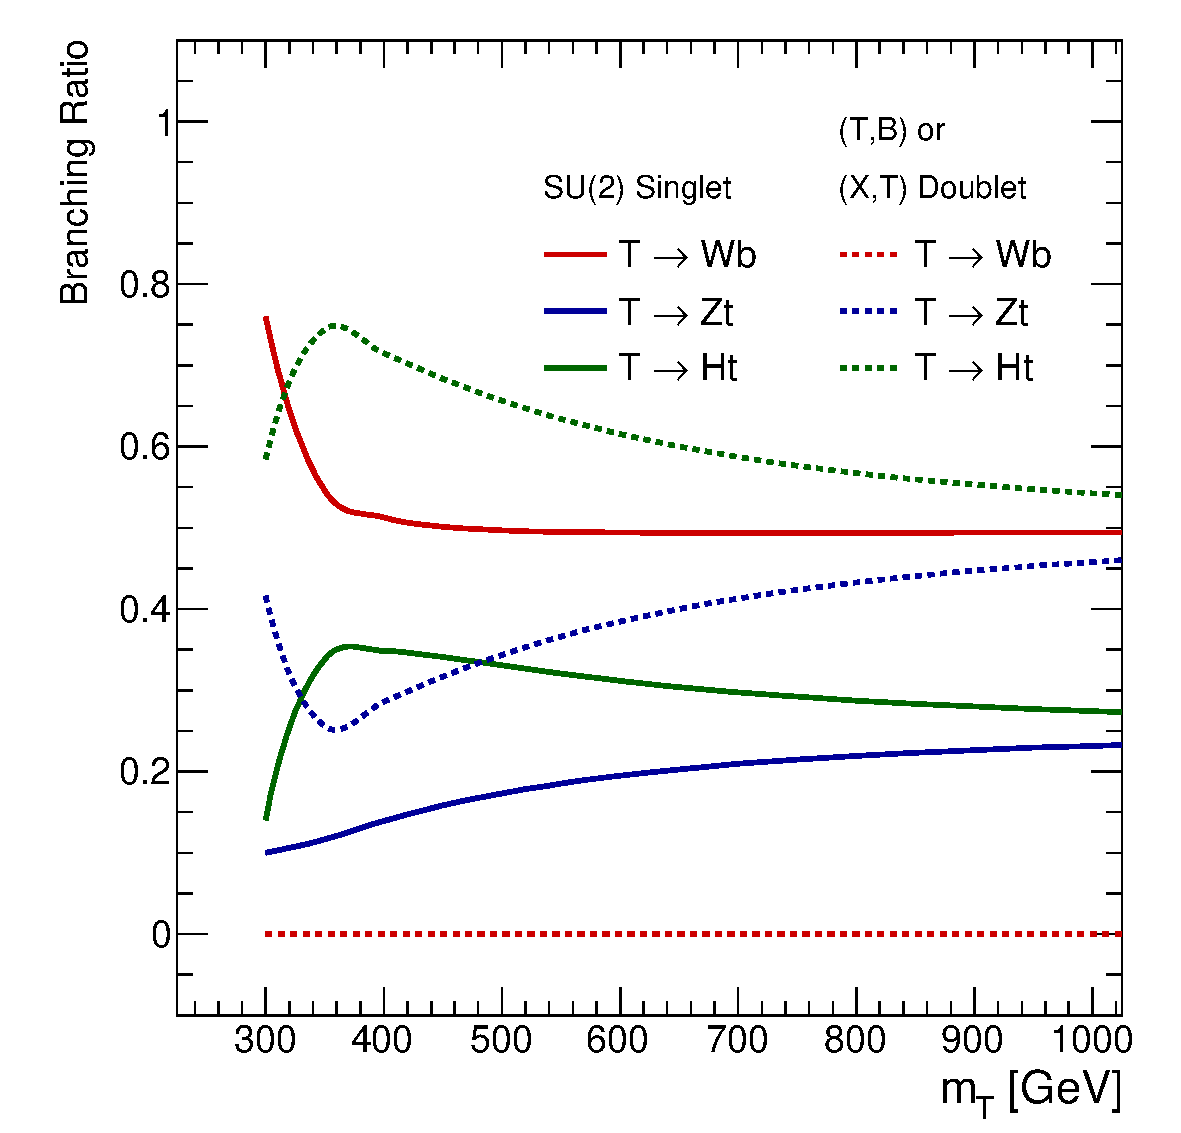
\includegraphics[width=0.9\textwidth]{figures/Theory/fig_02a.png}
  \caption{}
  \label{}
\end{subfigure}
\begin{subfigure}{0.5\textwidth}
  \centering
  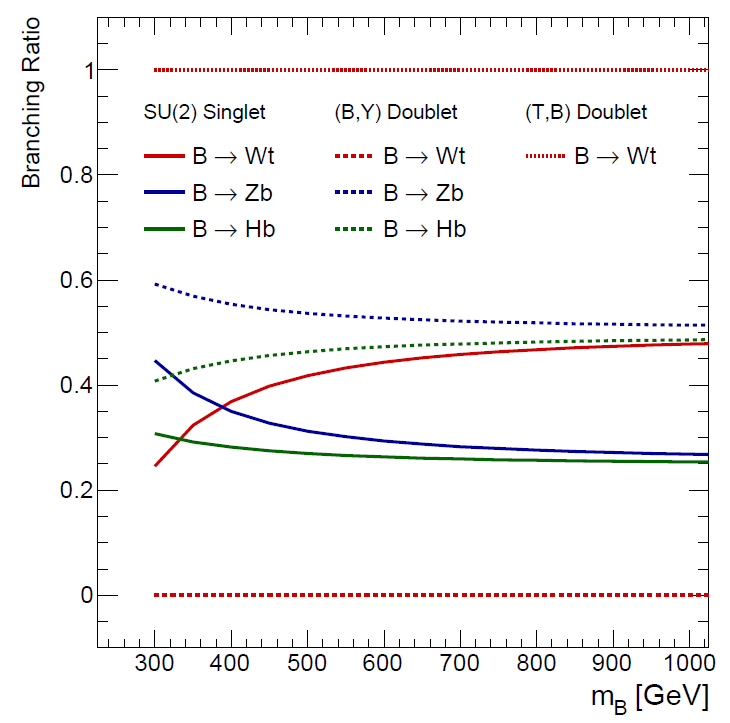
\includegraphics[width=0.9\textwidth]{figures/Theory/fig_02b.png}
  \caption{}
  \label{}
\end{subfigure}

\captionsetup{width=0.85\textwidth} \caption{\small Branching ratios for vector-like (a) top and (b) bottom partners as function of the heavy-quark mass $m_{T}$ and $m_{B}$ respectively for singlets and doublets. From reference \cite{Aguilar-Saavedra:2013qpa}.}
\label{fig:theo:VLQBRs}
\end{figure}

VLQs can be produced either in pairs through the strong interaction or as single quarks in association with SM quarks or bosons through the weak interaction \cite{Buchkremer:2013bha}.
Pair production is model independent since it just depends on the VLQ mass, while single production depends on the strength of VLQ coupling to SM quarks, and thus is model dependent. However, pair production suffers from a larger phase-space suppression with respect to single production, and if the VLQ mass is large enough ($\sim \tev$), single production may dominate over pair production. Example Feynman diagrams for pair and single production of a vector-like $T$-quark are shown in figure \ref{fig:theo:VLQprod}. Figure \ref{sec:theo:fig:vlqxsec} shows the cross section for pair production and single production in the $t$-channel as a function of VLQ mass.
\begin{figure}[h!]
\begin{subfigure}{0.5\textwidth}
  \centering
  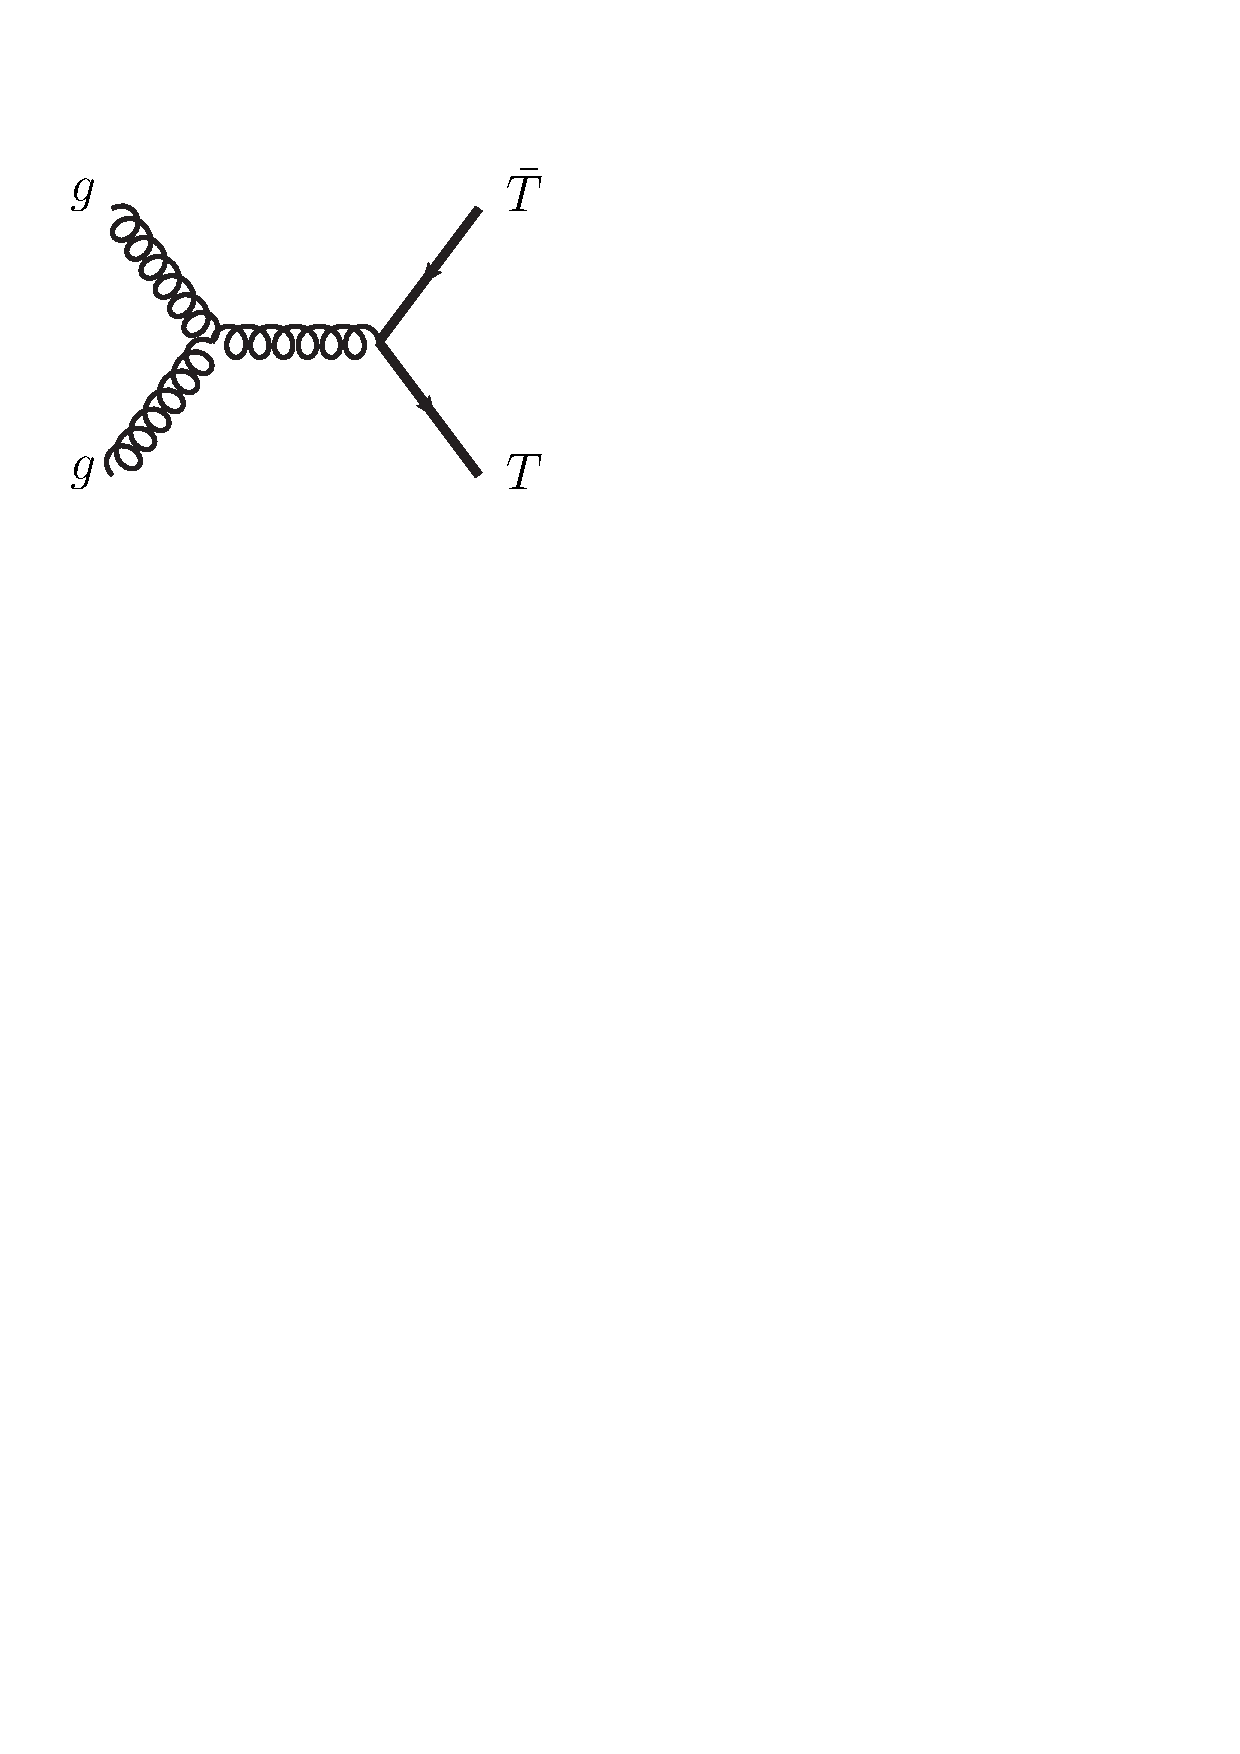
\includegraphics[width=0.6\textwidth]{figures/Theory/T_pairProd_good.pdf}
  \caption{}
  \label{}
\end{subfigure}
\begin{subfigure}{0.5\textwidth}
  \centering
  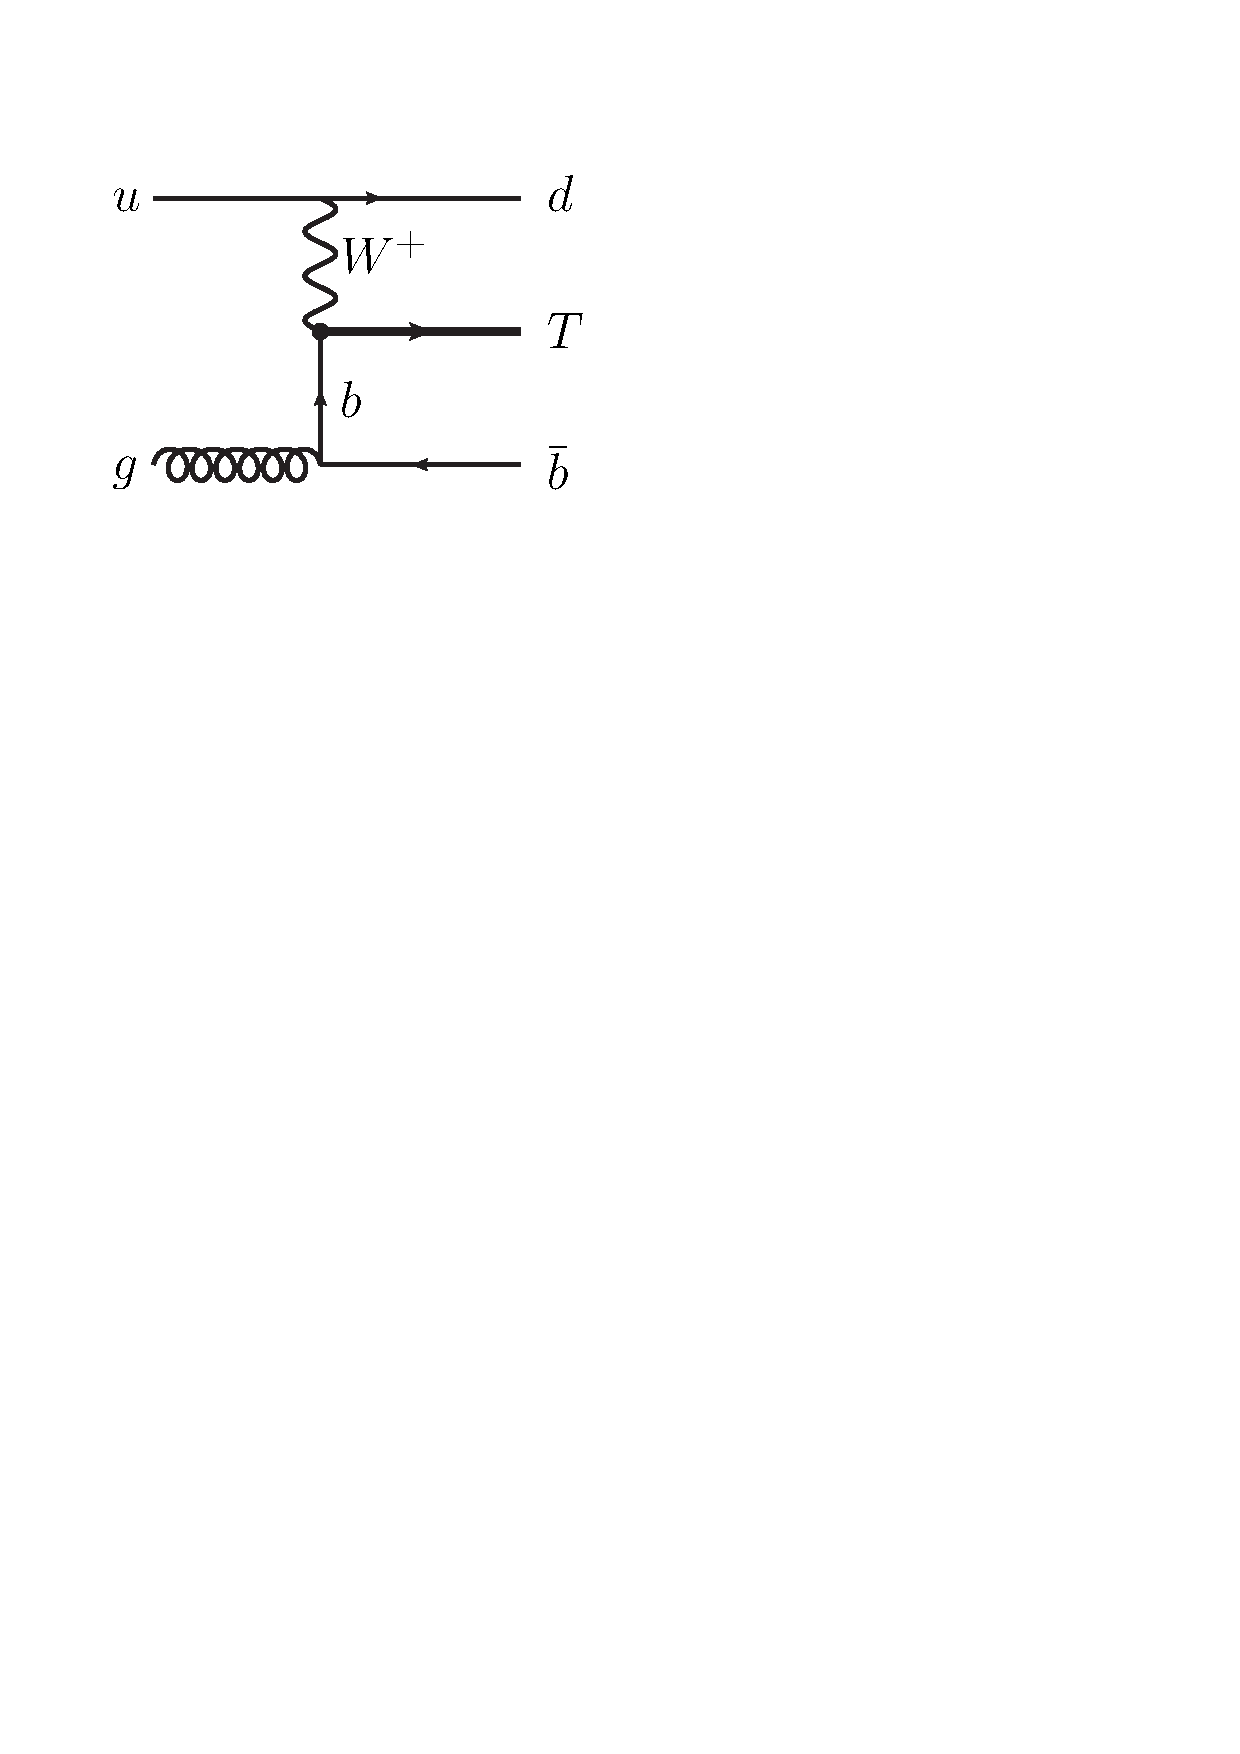
\includegraphics[width=0.6\textwidth]{figures/Theory/T_singleProd_good.pdf}
  \caption{}
  \label{}
\end{subfigure}

\captionsetup{width=0.85\textwidth} \caption{\small Representative leading-order Feynman diagrams for vector-like top (a) pair-production and (b) single-production modes.}
\label{fig:theo:VLQprod}
\end{figure}


\bfig[h!]
\centering
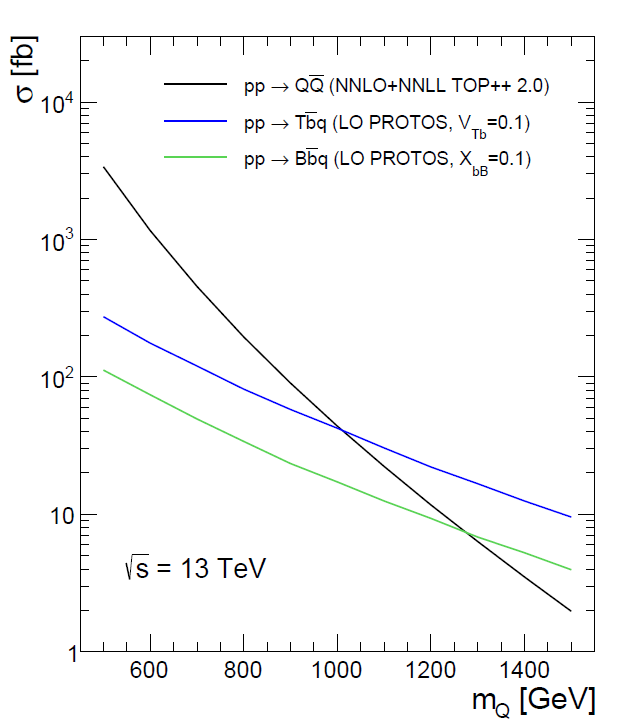
\includegraphics[width=0.4\textwidth]{figures/Theory/VLQxsec.png}
\captionsetup{width=0.85\textwidth} \caption{\small Production cross sections for pair and single production of VLQs in $pp$ collisions at $\sqrt{s}=$13 \tev. Pair production is computed at NNLO+NNLL order in QCD using {\sc Top++} 2.0 while single production is computed at LO in QCD with {\sc Protos} assuming $V_{Tb}=0.1$ and $X_{bB}=0.1$.}
\label{sec:theo:fig:vlqxsec}
\efig


\subsection{Anomalous four-top-quark production}
\label{sec:theo:fourtops}

The cross section of four-top-quark events predicted by the SM (see figure \ref{fig:theo:fourtopSM}) is extremely small, $\sigma_{t\bar{t}t\bar{t}}=9.2$ fb at $\sqrt{s} = 13$ $\tev$ \cite{Barger:1991vn}. 
However, in many BSM models, the four-top-quark production is enhanced, usually through the pair production of a new particle decaying to a top-antitop pair.\par
For example, a possible source of enhancement of the $t\bar{t}t\bar{t}$ cross-section appears in extra-dimensional models. In this framework the four-top-quark signal is an important probe for low-scale warped extra dimensions \cite{Jung:2010ms}; the enhancement comes from a heavy gluon that can be pair produced and decay into $\ttbar$ or via associate production of the heavy gluon with $t\bar{t}$. In flat-extra-dimensions models, such as 2UED/RPP, the enhancement is caused by the lightest particle of the tier (1,1), i.e. the vector photon $A_{\mu}^{(1,1)}$. In these models, to each SM fields corresponds a tower of massive resonances organised in tiers, labelled by two integers ($\ell$, $k$) that correspond to the discretised momenta along the extra dimensions. At leading order, all the states in each tier are degenerate with mass determined by the two integers:
\be
m^{2}=\frac{\ell^{2}}{R^{2}_{5}}+\frac{k^{2}}{R^{2}_{6}},
\ee 
\noindent where $R_{5}$ and $R_{6}$ are respectively the size of the two extra dimensions. For tier (1,1) its mass is given by $M^{(1,1)}=\sqrt{1/R^{2}_{5}+1/R^{2}_{5}}\sim \sqrt{2}M_{KK}$; assuming the two extra dimensions have the same size, and where $M_{KK}=M^{(0,1)}=M^{(1,0)}$.
The production of any heavy state of tier (1,1) contributes to the production of vector photons since it will undergo chain decays until the lightest state\footnote{The SM particles radiated in the chain decay are soft due to the typically small mass differences between states in the tier, and therefore will easily escape detection.} (see figure \ref{fig:theo:fourtopUED}). Therefore, the production cross section of vector photons can be sizeable even though their couplings to quarks and gluons are small.
The branching ratios of $A_{\mu}^{(1,1)}$ into SM particles are not predicted by the model, although the decay into $t\bar{t}$ is expected to be dominant \cite{Cacciapaglia:2011kz}.\par It is also possible to parametrise new physics, maybe not accessible at LHC, leading to four-top-quark production using the language of effective field theory with higher-dimensional operators.  This approach is used by composite top quark scenarios or RS models, in which, below the new physics scale, phenomena are described by an effective field theory containing the bound states of the new sector.
A dimension-six Lorentz-invariant operator with a four-point interaction (see figure \ref{fig:theo:fourtopEFT}) that involves only right-handed top quarks, $t_{R}$, can be considered:

\be
\mathcal{L}_{4t}=\frac{C_{4t}}{\Lambda^{2}}(\bar{t_{R}}\gamma_{\mu}t_{R})(\bar{t_{R}}\gamma_{\mu}t_{R}),
\ee 

\noindent where $\Lambda$ is the scale where new physics will manifest, and $C_{4t}$ is the effective coupling. The effective field theory approach is valid for $|C_{4t}|<16\pi^{2}$. In this framework right-handed top quarks are chosen because of the strong constraints coming from precision electroweak data on operators involving left-handed top quarks. 

\begin{figure}[t!]
\begin{subfigure}{0.33\textwidth}
  \centering
  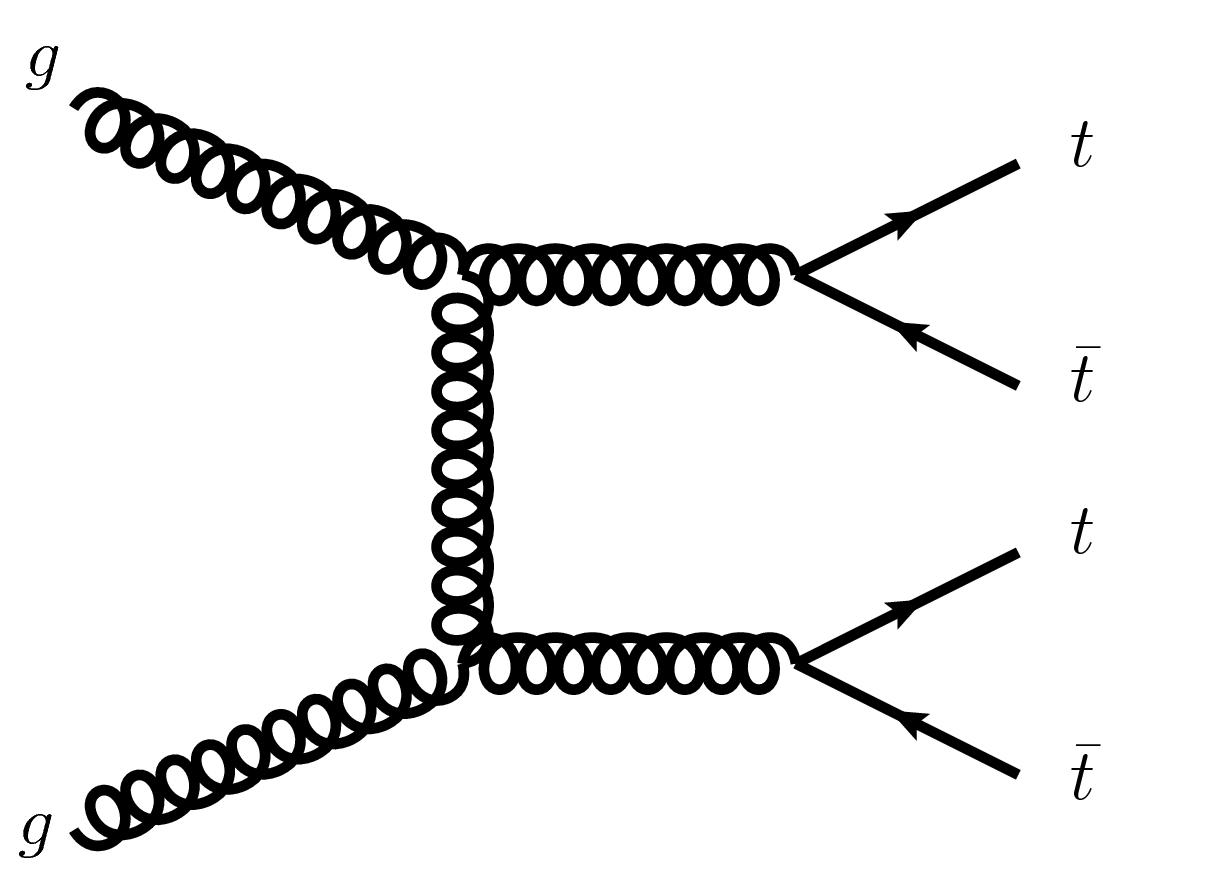
\includegraphics[width=0.8\textwidth]{figures/Theory/fig_03a.png}
  \caption{}
  \label{fig:theo:fourtopSM}
\end{subfigure}
\begin{subfigure}{0.33\textwidth}
  \centering
  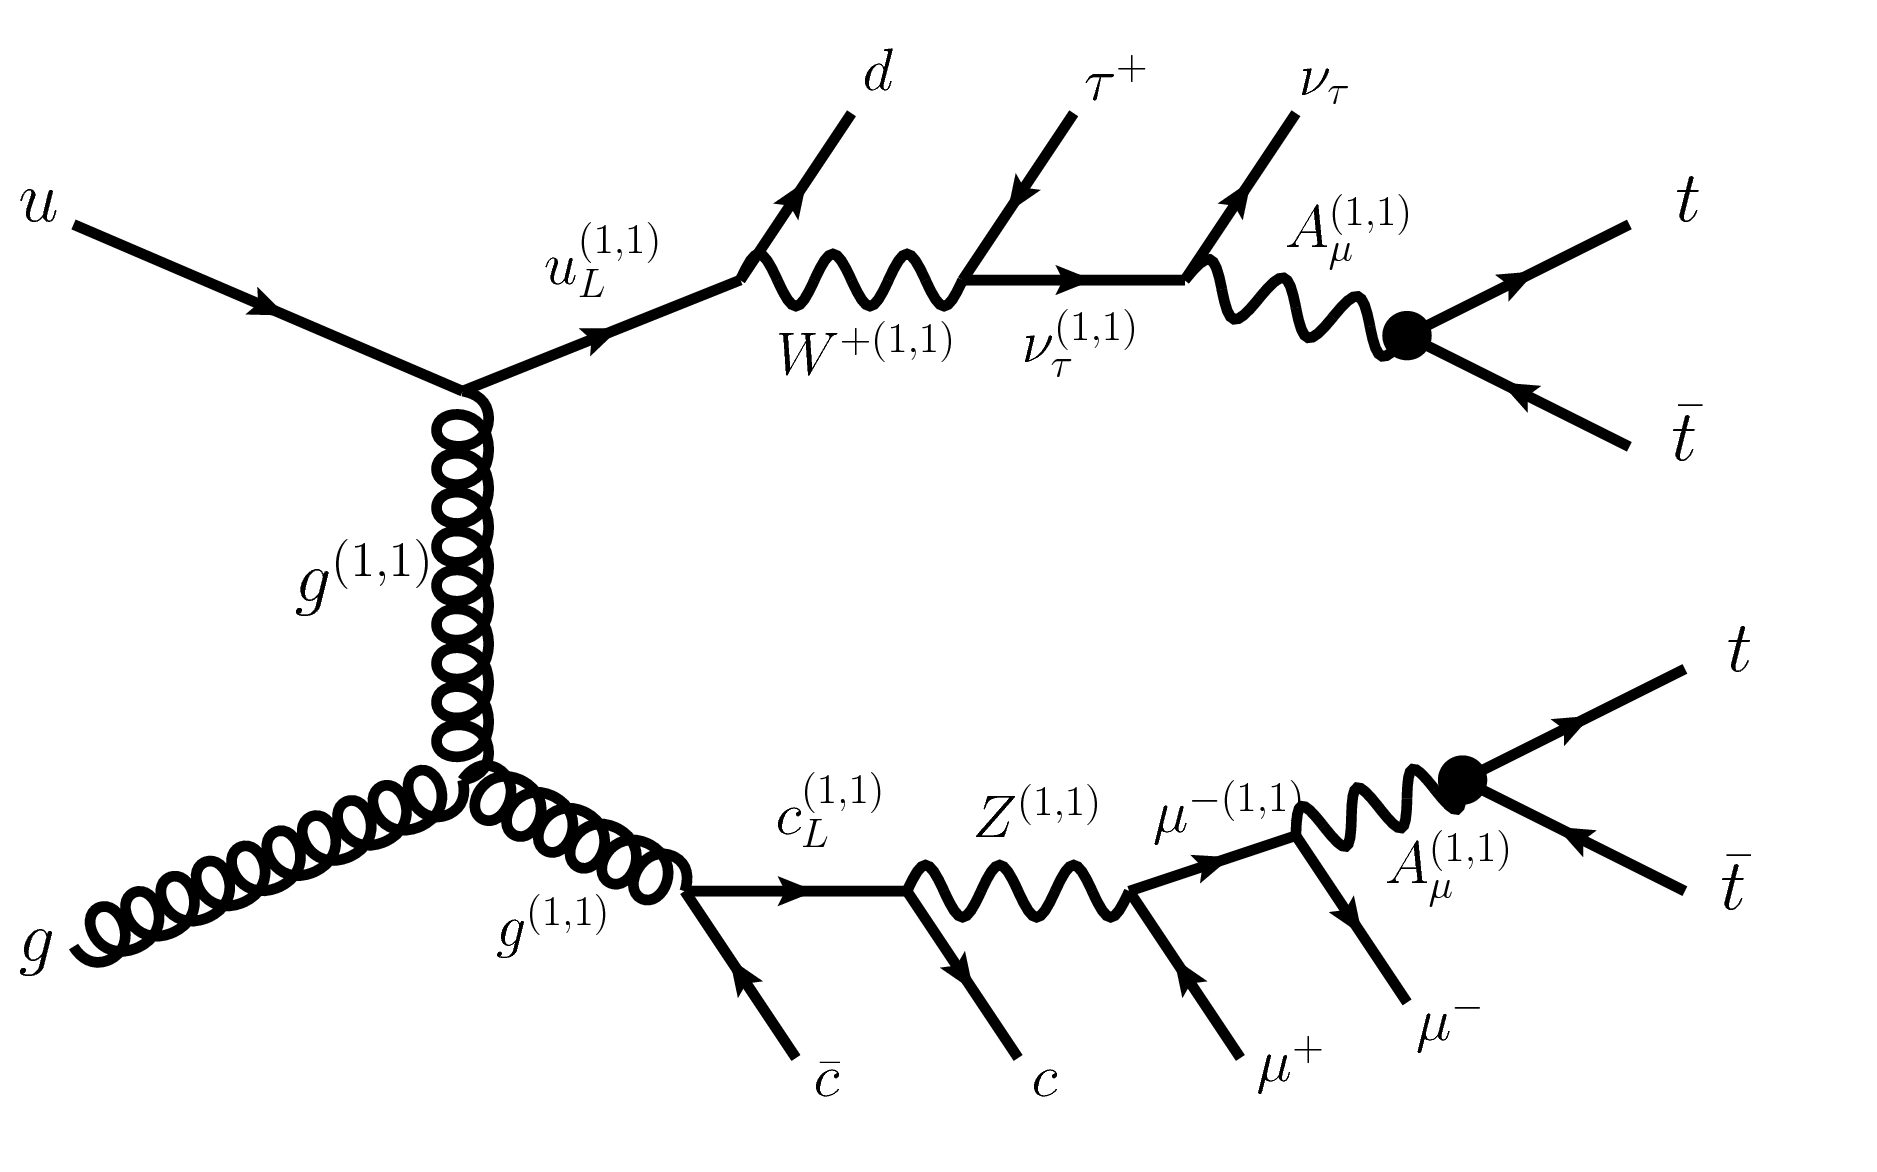
\includegraphics[width=1.15\textwidth]{figures/Theory/fig_03c.png}
  \caption{}
  \label{fig:theo:fourtopUED}
\end{subfigure}
\begin{subfigure}{0.33\textwidth}
  \centering
  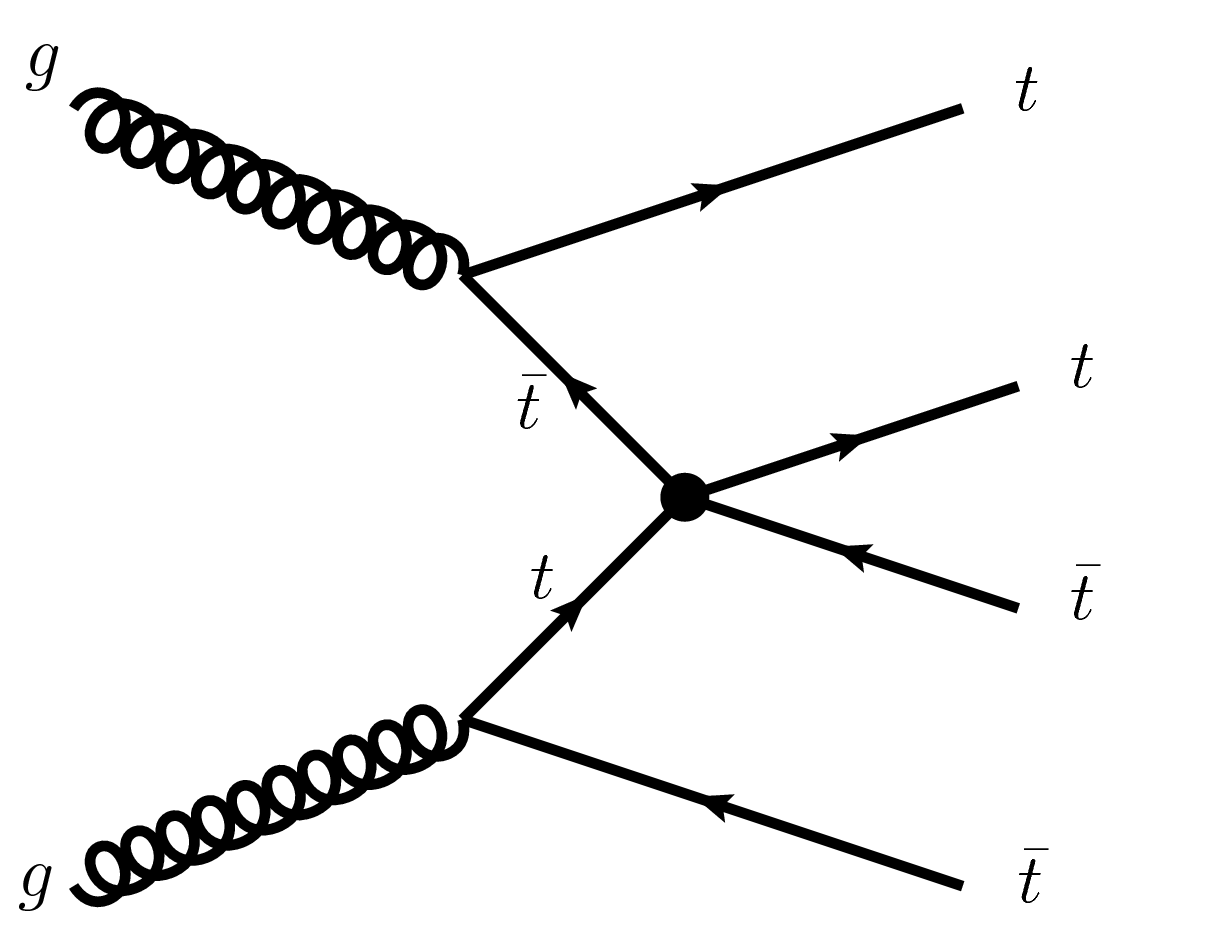
\includegraphics[width=0.75\textwidth]{figures/Theory/fig_03b.png}
  \caption{}
  \label{fig:theo:fourtopEFT}
\end{subfigure}


\captionsetup{width=0.85\textwidth} \caption{\small Representative leading-order Feynman diagrams for four-top-quark production within (a) the SM and several BSM scenarios: (b) via cascade decays from Kaluza-Klein excitations in a universal extra dimensions model with two extra dimensions compactified using the geometry of the real projective plane, and (c) via an effective four-top-quark interaction in an effective field theory model.}
\label{fig:theo:fourtop}
\end{figure}